%%%%%%%%%%%%%%%%%%%%%%%%%%%%%%%%%%%%%%%%%%%%%%%%%%%%%%%%%%%%%%%%%%
% Sample template for MIT Junior Lab Student Written Summaries
% Available from http://web.mit.edu/8.13/www/Samplepaper/sample-paper.tex
%
% Last Updated August 30, 2011
%
% Adapted from the American Physical Societies REVTeK-4.1 Pages
% at http://publish.aps.org
%
% ADVICE TO STUDENTS: Each time you write a paper, start with this
% template and save under a new filename. If convenient, don't
%    erase unneeded lines, just comment them out.  Often, they
%    will be useful containers for information.
%
% Using pdflatex, images must be either PNG, GIF, JPEG or PDF.
%     Turn eps to pdf using epstopdf.
%%%%%%%%%%%%%%%%%%%%%%%%%%%%%%%%%%%%%%%%%%%%%%%%%%%%%%%%%%%%%%%%%%


%%%%%%%%%%%%%%%%%%%%%%%%%%%%%%%%%%%%%%%%%%%%%%%%%%%%%%%%%%%%%%%%%%
% PREAMBLE
% The preamble of a LaTeX document is the set of commands that precede
% the \begin{document} line.  It contains a \documentclass line
% to load the REVTeK-4.1 macro definitions and various \usepackage
% lines to load other macro packages.
%
% ADVICE TO STUDENTS: This preamble contains a suggested set of
% class options to generate a ``Junior Lab'' look and feel that
% facilitate quick review and feedback from one's peers, TA's
% and section instructors. Don't make substantial changes without
%     first consulting your section instructor.
%%%%%%%%%%%%%%%%%%%%%%%%%%%%%%%%%%%%%%%%%%%%%%%%%%%%%%%%%%%%%%%%%%

\documentclass[aps,twocolumn,secnumarabic,balancelastpage,amsmath,amssymb,nofootinbib]{revtex4}
%\documentclass[aps,twocolumn,secnumarabic,balancelastpage,amsmath,amssymb,nofootinbib]{revtex4-1}
\pdfpagewidth 8.5in
\pdfpageheight 11in

%N.B. - Different computers have different packages installed. To compile this template in the current
% Athena environment, REVTeX 4.1 must be used. To use the older REVTeX 4, use the commented out
% Documentclass instead. If you are unable to compile the template at all, you
% may need to update your LaTeX packages. Don't hesitate to speak with your section instructor or a
% TA if you're having issues getting this template to compile.
% Documentclass Options
% aps, prl stand for American Physical Society and Physical Review Letters respectively
    % twocolumn permits two columns, of course
% nobalancelastpage doesn't attempt to equalize the lengths of the two columns on the last page
% as might be desired in a journal where articles follow one another closely
% amsmath and amssymb are necessary for the subequations environment among others
% secnumarabic identifies sections by number to aid electronic review and commentary.
% nofootinbib forces footnotes to occur on the page where they are first referenced
        % and not in the bibliography
% REVTeX 4.1 is a set of macro packages designed to be used withLaTeX 2e.
% REVTeX is well-suited for preparing manuscripts for submissionto APS journals.
       


\usepackage{lgrind} % convert program listings to a form includable in a LaTeX document
\usepackage{chapterbib} % allows a bibliography for each chapter(each labguide has it's own)
\usepackage{color} % produces boxes or entire pages with coloredbackgrounds
\usepackage{graphics}      % standard graphics specifications
\usepackage[pdftex]{graphicx} % alternative graphics specifications
\usepackage{longtable}     % helps with long table options
\usepackage{epsf} % old package handles encapsulated post scriptissues
\usepackage{bm}            % special 'bold-math' package
%\usepackage{asymptote} % For typesetting of mathematical illustrations
\usepackage{thumbpdf}
\usepackage[colorlinks=true]{hyperref} % this package should be added after all others
% use as follows: \url{http://web.mit.edu/8.13}
\usepackage{multirow}
\usepackage{subfigure}

% Define a useful new command for writing units
\newcommand{\cd}{$\cdot$}

%
% And now, begin the document...
%

\begin{document}
\title{Angular Dependence of Cosmic Ray Muon Flux}
\author{Stephen L.\ Eltinge and Jay M.\ Lawhorn}
\email{seltinge@mit.edu; klawhorn@mit.edu}
\date{\today}
\affiliation{MIT Department of Physics}

\begin{abstract}
We will measure the zenith angle dependence of the cosmic ray muon flux using a pair of scintillator counters with photomultiplier tube readouts on opposing ends. The angular dependence is known to go approximately with $\cos^2(\theta)$, where $\theta$ is measured from the zenith angle. We will test this prediction and make a measurement of the total cosmic ray muon rate.
\end{abstract}

\maketitle

The interaction of cosmic rays with particles in the upper atmosphere produces secondary showers of highly energetic particles, including neutrons, charged pions, and kaons. As shown in Figure \ref{fig:muon_shower}, many of the pions then decay into muons. The muon's mean lifetime is approximately 2.2 $\mu$s in its rest frame, but relativistic effects on high energy muons such as those produced in secondary showers allow them to easily penetrate the atmosphere and even some distance into the earth.

The Cosmic Ray Muon experiment \cite{spatrick} measures the velocity of cosmic ray muons via time of flight measurements and their mean lifetime. The combination of these two measurements provide evidence for relativistic time dilation. The apparatus for that experiment consists of two large rectangular scintillating paddles with one photomultiplier tube (PMT) read out per paddle. 

\begin{figure}[htb]
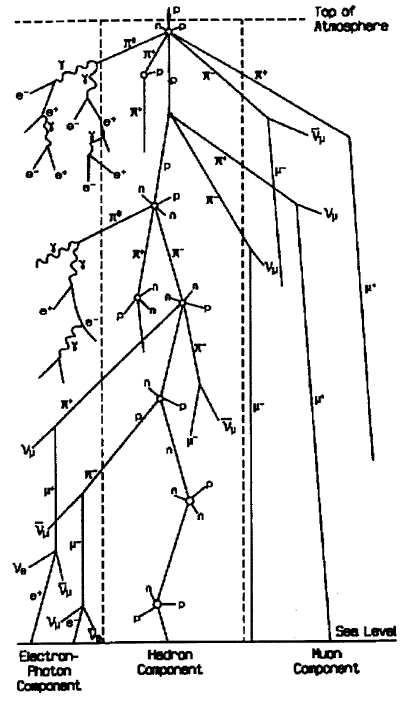
\includegraphics[width=7cm]{muon_shower.png}
\caption{Figure showing the production of muons and other particles from cosmic rays. From\cite{grieder}.}
\label{fig:muon_shower}
\end{figure}

The 8.13 apparatus has extremely poor resolution for the point of interaction, so the acceptance calculation is generally made over the expected zenith angle distribution of the cosmic ray muons, which is given as a $\cos^2(\theta)$ dependence. 

According to Grieder \cite{grieder}, the cosmic muon intensity as a function of zenith angle goes as 
\begin{equation}
\label{eqn:cosn}
I(\theta)=I(0^\circ)\cos^{n}(\theta),
\end{equation} 
where $n$ is a function of momentum. Grieder gives measured values of $n$ ranging from 1.6 to 3.3 for various latitudes and momentum thresholds.

Previous work on this problem using a similar setup \cite{kuo} indicates that we will measure an $n$ value close to 2.0. However, this work found that for angles near $\pm90^\circ$ the muon flux does not go to zero, instead exhibiting a small residual ``tail." 

We will use a pair of AMS scintillator counters, each of which consists of a long and narrow piece of scintillating material with a triad of PMTs at each end. We will read out each set of PMTs by oscilliscope. The apparatus itself is shown in Figure \ref{fig:apparatus}.

\begin{figure}[htb]
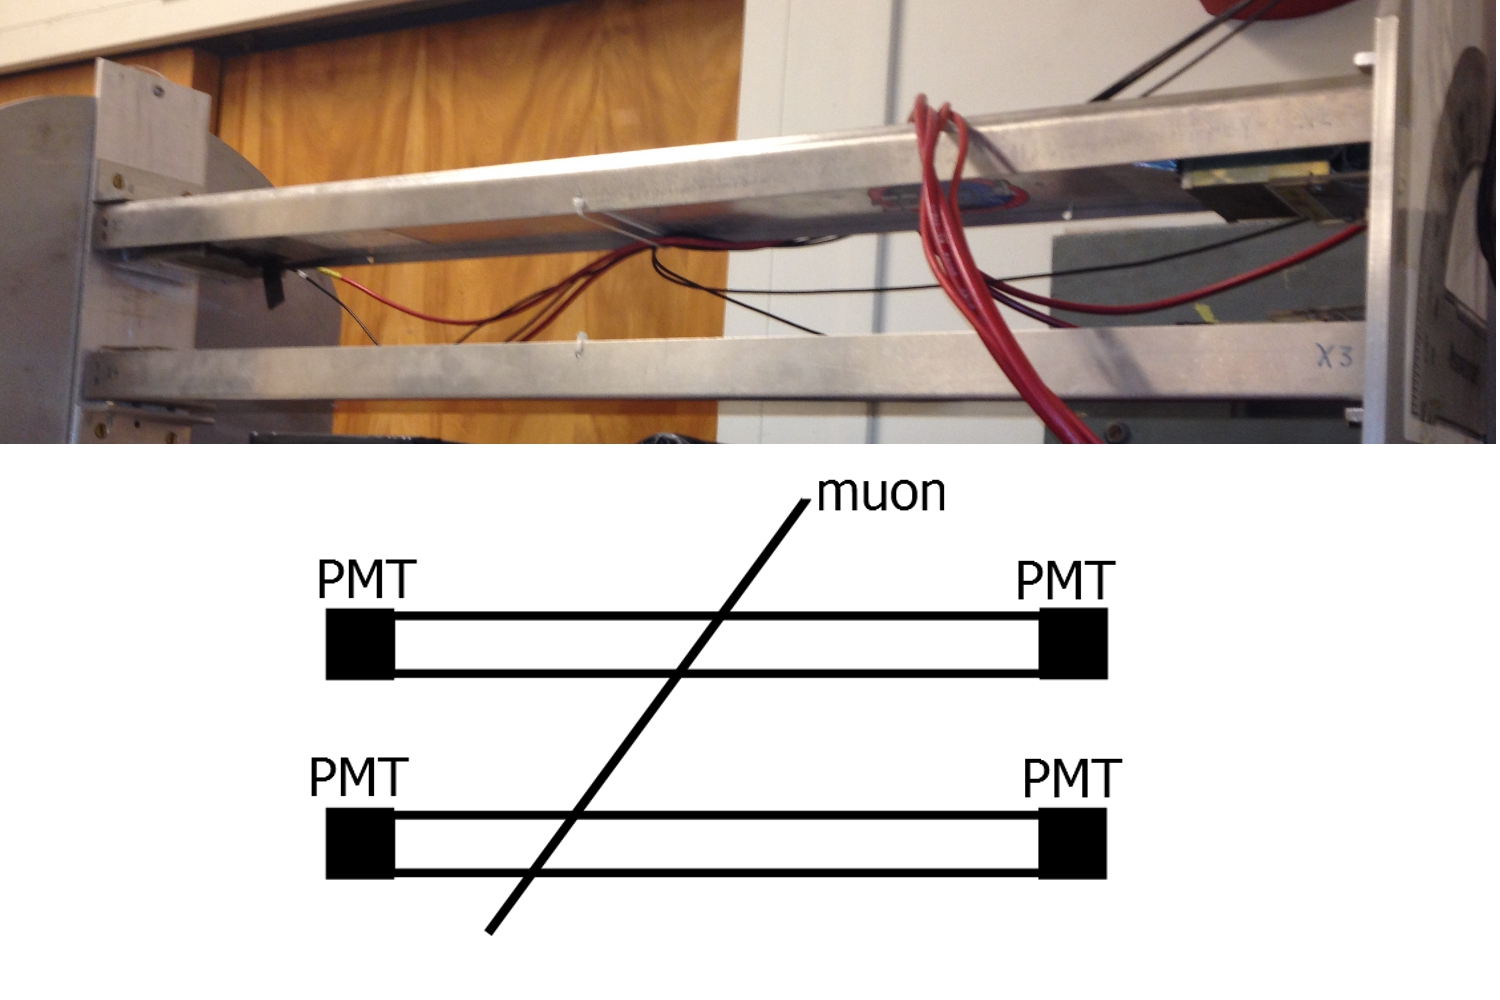
\includegraphics[width=7cm]{apparatus2.JPG}
\caption{(top) The two vertical bars each enclose one scintillator counter, with four total PMT readouts located on each end of the vertical bars. (bottom) Schematic of setup, with a muon path indicated. }
\label{fig:apparatus}
\end{figure}

The scintillation light produced by a muon interacting with the material will propagate and be detected at each end, and the time difference between detection at each end allows reconstruction of the point of interaction. Using a pair of these counters will allow us to reconstruct a flight path for each muon and ultimately an angle of incidence.

We will establish a working bias voltage for the PMTs by measuring the signal frequency as a function of bias voltage. If the bias voltage is too low, we will be losing events that we could otherwise detect. However, if the bias voltage is set too high, our signal will be dominated by amplified noise. We will set bias voltages for each PMT in the plateau between these two regimes.

We will measure the counter detection efficiency by placing two smaller scintillator paddles directly above and below one of the scintillator counters and looking at events where the two smaller paddles register a hit. The percentage of these events in which the middle counter also registers a hit will allow us to calculate the efficiency of the middle counter independently of the efficiencies of the smaller paddles. This setup will also allow us to validate our reconstruction of the point of interaction in the scintillator counter to a certain extent, although the expected precision in point of interaction will likely be much smaller than the additional paddles.

In order to find the angular dependence distribution, we will take data using the four PMT readouts in a series of long integration time runs, and reconstruct the flight path for each detected muon. The angle of incidence with respect to the azimuth can then be calculated. However, we will also need to take into account the geometric acceptance of the pair of scintillator counters, which we will model using a monte carlo simulation. If time permits, we will add detector effects and efficiencies to the simulation using either GEANT4 or a numerical integration scheme.

We will require the pair of AMS scintillator counters, a four-channel USB-capable osciliscope, and if possible, two similarly sized scintillator paddles to be used for efficiency measurements. We hope to borrow the osciliscope from junior lab, and all scintillators from Prof. Becker.

%%%%%%%%%%%%%%%%%%%%%%%%%%%%%%%%%%%%%%%%%%%%%%%%%%%%%%%%%%%%%%%%%%%%%%%%%%%%%
% Place all of the references you used to write this paper in a file
% with the same name as following the \bibliography command
%%%%%%%%%%%%%%%%%%%%%%%%%%%%%%%%%%%%%%%%%%%%%%%%%%%%%%%%%%%%%%%%%%%%%%%%%%%%%

\bibliography{SE_JL_proposal}


\end{document}
